\documentclass{article}
\usepackage[utf8]{inputenc}
\newcommand{\ihat}{\mathbf {\hat \imath}}
\newcommand{\jhat}{\mathbf {\hat \jmath}}
\usepackage{graphicx}

\begin{document}
\section*{Test 2}
\section*{1.A}
$$ \vec{P} = [x(t)]\, \ihat + [y(t)], \jhat $$
$$ \vec{P} = [\int x'(t)dt] \, \ihat + [\int y'(t)dt +y_0] \, \jhat $$
$$ \vec{P} = [\frac{1}{(t+1)^2} +C_x] \, \ihat + [\tanh(t)+C_y] \, \jhat $$

Solve $C_x$
$$\frac{1}{(0+1)^2} +C_x = 1$$
$$1 +C_x = 1$$
$$C_x = 0$$

Solve $C_y$
$$\tanh(0) +C_y = 0$$
$$0 +C_y = 0$$
$$C_y = 0$$

Final vector is 
$$ \vec{P} = [\frac{1}{(t+1)^2}] \, \ihat + [\tanh(t)] \, \jhat $$

\section*{1.C}
The point never stops moving, as the velocity in the x direction, given by $x'(t)$ can never equal 0, as shown below
$$0=- \frac{2}{(t+1)^2} $$
$$0*(t+1)^2 = - (t+1)^2* \frac{2}{(t+1)^2} $$
$$0 = -2 $$

\section*{1.D}
If the point moves through a finite distance, the distance it moves through must converge as T approaches infinity.
\\
Approximating the distance as a single segment yields
$$ \sqrt{x^2+y^2} $$
$$ \sqrt{[ \lim_{a\to\infty} \int_0^{a} x'(t)dt]^2+[ \lim_{b\to\infty} \int_0^{b} y'(t)dt]^2} $$
$$ \sqrt{[ \lim_{a\to\infty} \frac{1}{(t+1)^2}|_0^a]^2+[ \lim_{b\to\infty} \frac{e^x-e^{-x}}{e^x+e^{-x}}|_0^{b}]^2} $$
Evaluating yields
$$ \sqrt{[ 0 - 1]^2+[ 1-0]^2} $$
$$ \sqrt{2} $$

\section*{2.D}

From part C, the non-parametric equation was determined to be $y=1-2x^2$. Therefore, it should be a graph of that parabola, but range and domain restricted to $[-1,1]$ because of the bounds of the sine and cosine functions
\begin{center}
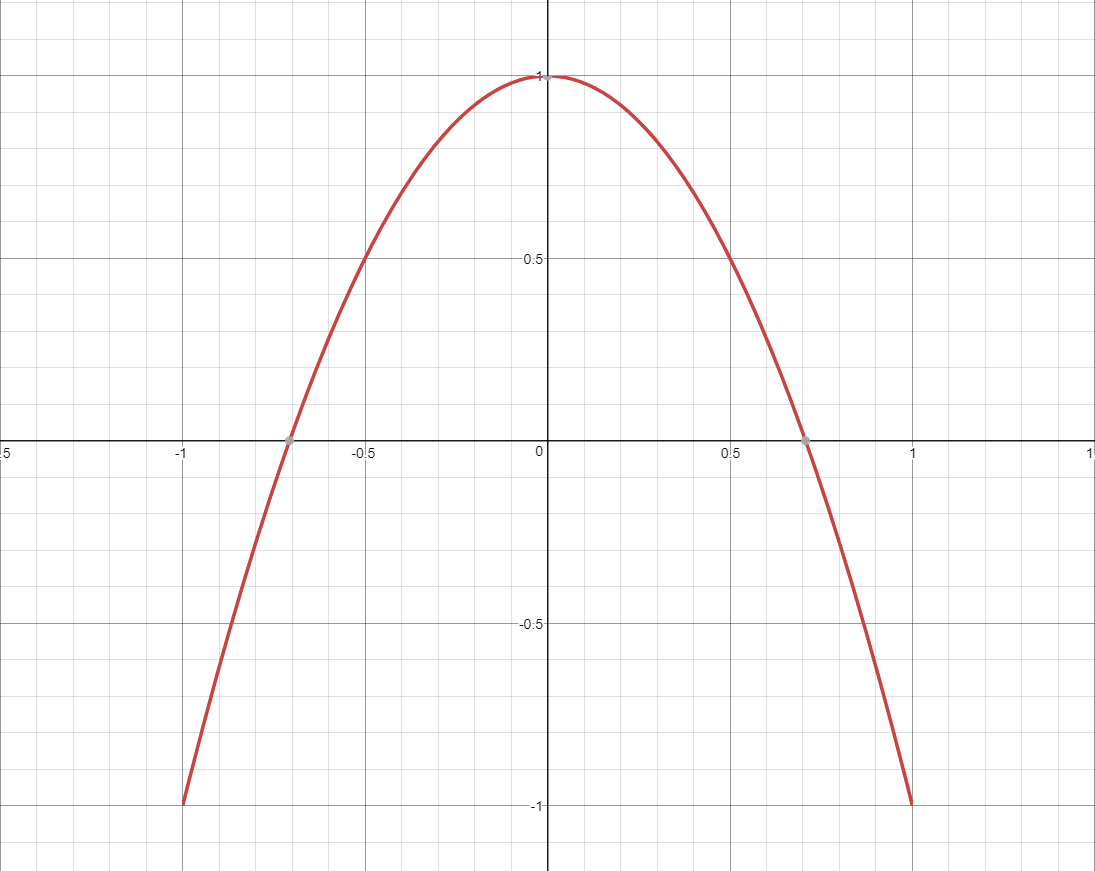
\includegraphics[width=\linewidth]{graph.png}
\end{center}

\end{document}
